\documentclass[12pt, oneside, titlepage]{article}   	% use "amsart" instead of "article" for AMSLaTeX format

\usepackage{graphicx}
\graphicspath{ {\string} }
\usepackage{subcaption}

\usepackage{tabularx}   

%%%%%%%%%%%%%%%%%%%%%%%%%%%%%%%%%%%%%%%%%%%%%%%%%%%%
% set up packages
%%%%%%%%%%%%%%%%%%%%%%%%%%%%%%%%%%%%%%%%%%%%%%%%%%%%
\usepackage{geometry}                
\usepackage{textcomp}                
\usepackage{amsmath}                
\usepackage{graphicx}                
\usepackage{amssymb}                
\usepackage{fancyhdr}                
\usepackage{subcaption}                
\usepackage{bm}                
\usepackage{lineno}
% package for comments
\usepackage{soul}
\sethlcolor{lightgray}

\usepackage{wrapfig}

\usepackage[usenames, dvipsnames]{color}

\usepackage[breaklinks=true]{hyperref}
\hypersetup{
    colorlinks=true,
    linkcolor=red,
    filecolor=orange,      
    urlcolor=red,
    citecolor=Violet,
}

\usepackage[superscript,noadjust]{cite} % puts dash in citations to abbreviate
\usepackage [autostyle, english = american]{csquotes} % sets US-style quotes

\usepackage{etoolbox} % block quotes

\usepackage{float}

\usepackage{pgf}
\usepackage{tikz}
\usepackage{eqnarray}

\usepackage{listings} % code blocks
\usepackage{setspace}

\usepackage{lscape}

\usepackage{natbib}
%\bibliographystyle{abbrvnat}
\setcitestyle{authoryear}

% Adds parentheses around year
%\setcitestyle{authoryear,open={(},close={)}}

%%%%%%%%%%%%%%%%%%%%%%%%%%%%%%%%%%%%%%%%%%%%%%%%%%%%
% call packages
%%%%%%%%%%%%%%%%%%%%%%%%%%%%%%%%%%%%%%%%%%%%%%%%%%%%	
\geometry{letterpaper, marginparwidth=60pt} % sets up geometry              		
\linenumbers % adds line numbers 
\MakeOuterQuote{"} % sets quote style
\doublespacing % setspace

%%%%%%%%%%%%%%%%%%%%%%%%%%%%%%%%%%%%%%%%%%%%%%%%%%%%
% patches with etoolbox 
%%%%%%%%%%%%%%%%%%%%%%%%%%%%%%%%%%%%%%%%%%%%%%%%%%%%	
% block quotes
\AtBeginEnvironment{quote}{\small}

% linenumbers
\makeatletter
\patchcmd{\@startsection}{\@ifstar}{\nolinenumbers\@ifstar}{}{}
\patchcmd{\@xsect}{\ignorespaces}{\linenumbers\ignorespaces}{}{}
\makeatother

%%%%%%%%%%%%%%%%%%%%%%%%%%%%%%%%%%%%%%%%%%%%%%%%%%%%
% tikzlibrary modifications
%%%%%%%%%%%%%%%%%%%%%%%%%%%%%%%%%%%%%%%%%%%%%%%%%%%%	
\usetikzlibrary{fit}
\usetikzlibrary{positioning}
\usetikzlibrary{arrows}
\usetikzlibrary{automata}

%%%%%%%%%%%%%%%%%%%%%%%%%%%%%%%%%%%%%%%%%%%%%%%%%%%%
% page formatting; exact 1 in margins
%%%%%%%%%%%%%%%%%%%%%%%%%%%%%%%%%%%%%%%%%%%%%%%%%%%%
\pagestyle{plain}                                                     

\setlength{\textwidth}{6.5in}    
\setlength{\oddsidemargin}{0in}
\setlength{\evensidemargin}{0in}
\setlength{\textheight}{8.5in}
\setlength{\topmargin}{0in}
\setlength{\headheight}{0in}
\setlength{\headsep}{0in}
\setlength{\footskip}{.5in}

%%%%%%%%%%%%%%%%%%%%%%%%%%%%%%%%%%%%%%%%%%%%%%%%%%%%
% defining code blocks using listings package
%%%%%%%%%%%%%%%%%%%%%%%%%%%%%%%%%%%%%%%%%%%%%%%%%%%%

\definecolor{dkgreen}{rgb}{0,0.6,0}
\definecolor{gray}{rgb}{0.5,0.5,0.5}
\definecolor{mauve}{rgb}{0.58,0,0.82}

\lstset{frame=tb,
  language=R,
  aboveskip=3mm,
  belowskip=3mm,
  showstringspaces=false,
  columns=flexible,
  basicstyle={\small\ttfamily},
  numbers=none,
  numberstyle=\tiny\color{gray},
 % keywordstyle=\color{blue},
  commentstyle=\color{dkgreen},
  stringstyle=\color{mauve},
  breaklines=true,
  breakatwhitespace=true,
  tabsize=3,
  otherkeywords={0,1,2,3,4,5,6,7,8,9},
  deletekeywords={data,frame,length,as,character,dunif,ps},
}

%%%%%%%%%%%%%%%%%%%%%%%%%%%%%%%%%%%%%%%%%%%%%%%%%%%%
%%%%%%%%%%%%%%%%%%%%%%%%%%%%%%%%%%%%%%%%%%%%%%%%%%%%
% begin document
%%%%%%%%%%%%%%%%%%%%%%%%%%%%%%%%%%%%%%%%%%%%%%%%%%%%
%%%%%%%%%%%%%%%%%%%%%%%%%%%%%%%%%%%%%%%%%%%%%%%%%%%%

\begin{document}

%%%%%%%%%%%%%%%%%%%%%%%%%%%%%%%%%%%%%%%%%%%%%%%%%%%%
% TITLE PAGE
%%%%%%%%%%%%%%%%%%%%%%%%%%%%%%%%%%%%%%%%%%%%%%%%%%%%
\begin{titlepage}
   \begin{center}
       \vspace*{1cm}
 
       \textbf{Intraspecific variation in range-wide seed bank dynamics is not consistent with density-independent bet hedging alone}
 
       \vspace{1.5cm}
 
       Gregor-Fausto Siegmund and Monica Geber
 
   	Last updated: \today
	

	
 
   \end{center}
\end{titlepage}
%

%%%%%%%%%%%%%%%%%%%%%%%%%%%%%%%%%%%%%%%%%%%%%%%%%%%%
% INTRODUCTION
%%%%%%%%%%%%%%%%%%%%%%%%%%%%%%%%%%%%%%%%%%%%%%%%%%%%
\section{Introduction}

Organisms across the tree of life exhibit life history strategies to persist in environments with different levels of variability, uncertainty, and predictability. In annual plants, interannual variation in fitness can favor the evolution of delayed germination and seed dormancy that establish soil seed banks. Seed banks can buffer plant populations against environmental change and stochasticity (\cite{eager2014,paniw2017}), increase effective population size (\cite{nunney2002,waples2006}), and maintain genetic diversity (\cite{mccue1998}). Theory thus suggests that seed banks have key ecological and evolutionary consequences (\cite{evans2005}). 

Evolutionary ecologists have classically theorized seed banks as a bet-hedging strategy that maximizes geometric mean fitness across years (reviewed in \cite{philippi1989,simons2011}). For populations that experience complete reproductive failure in some years--if no seedlings survive, or if seed set is zero--a seed bank prevents extinction. More generally, because long-term population growth is multiplicative, it is sensitive to variance in fitness from year to year. As a consequence, optimal bet-hedging strategies reduce variance in geometric mean fitness even if they decrease the arithmetic mean fitness (\cite{cohen1966}). The value of delaying germination also depends on how safe the seed bank is; if seed mortality is high, there is a greater risk to remaining in the soil (\cite{cohen1966}). Density-independent models have been expanded to density-dependent cases with competition, in which case seed banks are an evolutionary stable strategy (\cite{ellner1985,ellner1985a}). However, seed strategies are shaped by environments that vary in both their levels of uncertainty and predictability. Predictive germination is expected if seeds are able to detect and respond to cues that reliably predict fitness upon germination (\cite{cohen1967}). Ultimately, it is likely that life history strategies are the product of a combination of these factors (\cite{simons2011}), an idea supported by research carried out with a guild of Sonoran Desert annuals (\cite{venable2007,gremer2014,gremer2016}).

Empirical studies of intraspecific variation in seed dormancy and germination assess the predictions of bet-hedging theory in various ways. Common garden experiments with seeds collected across precipitation gradients test for positive correlations between germination and rainfall at the source population (e.g. \cite{hacker1984,hacker1989,philippi1993a,clauss2000}). Field studies over elevation gradients demonstrate clines in dormancy (e.g. \cite{fernandez-pascual2013}) and germination (\cite{gremer2020}). Finally, studies examine seed behavior over the course of multiple years to examine the relationship between delayed germination and environmental variability (e.g. \cite{philippi1993,evans2007}). However, the strongest tests of bet-hedging models have been interspecific comparisons that examine the contribution of delayed germination to population growth (\cite{venable2007,gremer2014,gremer2016}). To our knowledge, only two studies of intraspecific variation have focused on the consequences of delayed germination on population growth (\cite{clauss1999a,evans2007}). Here, we expand on this body of research by using a 15 year record of per-capita reproductive success across 20 populations to test whether the observed life history variation is consistent with bet-hedging theory. 
 
Populations of the winter annual \textit{Clarkia xantiana} ssp. \textit{xantiana} are distributed across a complex landscape in the southern Sierra Nevada Mountains (Fig.~\ref{fig:intro-figure}). Although earlier work suggested the species lacked a soil seed bank (\cite{lewis1962}), multiple lines of evidence now support the presence and relevance of a seed bank in populations of \textit{C. xantiana} ssp. \textit{xantiana}. In field experiments burying seeds in bags (\cite{eckhart2011}) and pots (\hl{Geber, unpublished data}), seeds can germinate at least up to 3 years after burial. Fifteen years of surveys suggest that the seed bank may allow some populations to persist exclusively as seeds for as long as 4 consecutive years (Fig.~\ref{fig:intro-figure}D). Seeds lack morphological adaptations for dispersal (\cite{knies2004}) and spatial distribution patterns in populations are consistent with dispersal limitation (\cite{kramer2011}). We thus expect limited seed dispersal among populations over the relatively short temporal scales reported in this study.

A previous study of \textit{C. xantiana} population dynamics identified a decrease in population growth rate from west to east across the species' distribution in the southern Sierra Nevada, CA (\cite{eckhart2011}). Germination rate of first-year seeds increased from west to east (\cite{eckhart2011}). Variability in rainfall during the growing season shows a similar pattern as germination, from less variable (and wetter) in the west to more variable (and drier) in the east (\cite{eckhart2011}; Fig.~\ref{fig:intro-figure}B\&C for pattern from 2005-2020). In addition to these spatial patterns, demographic observations \cite{eckhart2011} and transplant experiments demonstrate that fitness can exhibit dramatic interannual variation associated with rainfall (e.g. 30-fold between a wet and dry year in \cite{geber2005}). If high interannual variation in rainfall were associated with high interannual variation in fitness, lower germination would be favored eastern populations. This is the opposite of the observed pattern. The relationship between the environment and fitness may be complex, especially when multiple variables change over the study area or different parts of the life cycle may differ in how responsive they are to environmental variation. The variation in life history and climate observed among populations prompted us to consider whether bet-hedging might explain life history patterns in the species. In this study, we thus seek to understand intraspecific variation in \textit{C. xantiana} seed vital rates in the context of temporal variation in fitness.

Here, we test whether life history patterns in \textit{Clarkia xantiana} ssp. \textit{xantiana} are consistent with predictions made by bet-hedging models. We combine seed burial experiments and 15 years of observations on aboveground vital rates from 20 populations to address the following questions: (1) Is there a negative correlation between germination and seed survival (Fig.~\ref{fig:intro-figure}E)? (2) Is there a negative correlation between germination and variance in per-capita reproductive success (Fig.~\ref{fig:intro-figure}F)? (3) Is per-capita reproductive success positively correlated with growing season precipitation? (4) Does germination predicted by density-independent bet-hedging models match observed germination? Because we find that life history patterns are not consistent with predictions, we examined two additional pieces of evidence to explore support for complementary hypotheses: (5) Is there a correlation between variation in the environment and per-capita reproductive success? (6) What is the relative contribution of different fitness components to total variance in per-capita reproductive success?

%%%%%%%%%%%%%%%%%%%%%%%%%%%%%%%%%%%%%%%%%%%%%%%%%%%%
% METHODS
%%%%%%%%%%%%%%%%%%%%%%%%%%%%%%%%%%%%%%%%%%%%%%%%%%%%
\section{Methods}

\subsection{Clarkia life history}

\textit{Clarkia xantiana} ssp. \textit{xantiana} is a winter annual that germinates with late fall and winter rains. In our study region, the Kern Valley in the southern Sierra Nevada Mountains, germination historically happens from November and late February or early March. Seedlings grow throughout the winter and spring, and surviving plants flower in late spring and early summer, late April into mid June. Pollinated fruits set seed in the early summer, June to July. Seeds of \textit{C. xantiana} are produced in early summer, with fruits that dry out and gradually split open. Most seeds appear to be shed from fruits within 3-4 months after production, but can remain on the plant for up to a year. Seeds are small ($<1$ mm in width) and have no structures to aid in aerial dispersal. 

We represent the \textit{C. xantiana} life history in terms of transitions from October of year $t$ to October of year $t+1$. Transitions are the product of seed survival and germination, and aboveground seedling survival to fruiting, fruit production, and seeds per fruit. For this study, we assume that the new and old seeds differ in their survival rates in the seed bank, but do not include additional age structure and assume germination of new and old seeds is the same. We also we assume that all plants experience the same vital rates upon germination. We describe population growth rate by the following equation:

 \begin{align}
  \begin{split}
\lambda = g_1Y(t) s_0 s_1 + (1-g_1) s_2 s_3.  \label{eq:di-equation}
  \end{split}
\end{align}

Germination is given by $g_1$. Seed survival from seed production to the first October is $s_0$, and survival from October to February is $s_1$ and $s_3$ for age 0, and 1 seeds, respectively. Survival from February to October is given as $s_2$. Per-capita reproductive success in year $t$, $Y(t)$ is the product of seedling survival to fruiting, fruits per plant, and seeds per fruit.

\subsection{Creating the dataset}

We used field experiments and surveys to assemble observations of above- and below-ground demography for 20 populations of \textit{Clarkia xantiana} (Table \ref{tab:datasets}). A subset of the demographic data has been used to test hypotheses about the geography of demography (\cite{eckhart2011}) and species distributions (\cite{pironon2018}). Here, we use field surveys to collect data on seedling survival, fruit production, and seed set. We also conduct field experiments to observe emergence of seedlings and seeds remaining intact in the soil seed bank. We use the data from the surveys and experiments to estimate the demographic parameters that describe the life cycle (Equation~\ref{eq:di-equation}A\&B). Ultimately, we use these estimates to calculate germination, seed survival, and per-capita reproductive success to test predictions of bet-hedging models.

%
\begin{singlespace*}
\captionof{table}{ Summary of data sets used to estimate demographic parameters. } \label{tab:datasets} 
\begin{center}
%\documentclass[varwidth=\maxdimen,border=1pt]{standalone}
%                 
%\usepackage{bm}   
%\usepackage{tabularx}   
%
%\usepackage{caption}          
% \captionsetup[table]{labelfont=sc}
%
%\usepackage{amsmath}                      
%\usepackage{amssymb}      
%
%
%%%%%%%%%%%%%%%%%%%%%%%%%%%%%%%%%%%%%%%%%%%%%%%%%%%%%
%%%%%%%%%%%%%%%%%%%%%%%%%%%%%%%%%%%%%%%%%%%%%%%%%%%%%
%% begin document
%%%%%%%%%%%%%%%%%%%%%%%%%%%%%%%%%%%%%%%%%%%%%%%%%%%%%
%%%%%%%%%%%%%%%%%%%%%%%%%%%%%%%%%%%%%%%%%%%%%%%%%%%%%
%
%\begin{document}

%%%%%%%%%%%%%%%%%%%%%%%%%%%%%%%%%%
% DATASETS
%%%%%%%%%%%%%%%%%%%%%%%%%%%%%%%%%%

%\captionof{table}{ Summary of data sets used to estimate parameters. } \label{tab:title1} 
  \begin{tabularx}{\linewidth}{ l l c c } 
 \hline
 \hline
\multicolumn{1}{ c }{ Parameter data } & 
\multicolumn{1}{ c }{ Description } & 
\multicolumn{1}{ c }{ Data set }  & 
\multicolumn{1}{ c }{ Time span } \\
 \hline
 % seed bag burial experiment
 \textsc{Seed vital rates} & --- & --- & --- \\ 
 Seed survival and germination & Seed bag burial & $\bm{\mathrm{Y}}_1$ & 2006-2009  \\ 
 Seed viability & Viability trials & $\bm{\mathrm{Y}}_2$ & 2006-2009 \\ 
 Seed survival and germination & Seed pots & $\bm{\mathrm{Y}}_3$ & 2013-2019  \\ 
 \textsc{Seedling survival} & --- & --- & --- \\ 
 Seedling survival to fruiting & Field surveys & $\bm{\mathrm{Y}}_4$ & 2006-2019 \\ 
 \textsc{Fruits per plant} & --- & --- & --- \\ 
 Total fruit equivalents per plant & Field surveys & $\bm{\mathrm{Y}}_5$ & 2006-2012 \\ 
 Undamaged and damaged fruits per plant & Field surveys & $\bm{\mathrm{Y}}_6$ & 2013-2019 \\ 
 Total fruit equivalents per plant & Extra plots & $\bm{\mathrm{Y}}_7$ & 2006-2012 \\ 
 Undamaged and damaged fruits per plant & Extra plots & $\bm{\mathrm{Y}}_8$ & 2013-2019 \\ 
 \textsc{Seeds per fruit} & --- & --- & --- \\ 
  Seeds per undamaged fruit & Lab counts & $\bm{\mathrm{Y}}_9$ & 2006-2019 \\ 
  Seeds per damaged fruit & Lab counts & $\bm{\mathrm{Y}}_{10}$ & 2013-2019 \\   
  \hline
\end{tabularx} 
%\end{document}
\end{center}
\end{singlespace*} 

\subsubsection{Field surveys for aboveground components of demography}

We conducted field surveys of seedlings, fruiting plants, fruits per plant, and seeds per fruit at two spatial scales (Figure~\ref{fig:diagram}A; \cite{eckhart2011}). First, in October 2005, one of us (MAG) established 30 $1\times0.5$ m$^2$ permanent plots at each of the 20 study populations. The permanent plots were arrayed across four to six transects per site, and each plot was 2.5 m apart along a transect. Permanent plots were used for annual surveys of seedlings, fruiting plants, and fruits per plant. Second, additional, haphazardly distributed $1\times0.5$ m$^2$ plots were used each year to supplement estimates of fruits per plant from permanent plots, and to identify plants for fruit collection. By collecting fruits from plants outside the permanent plots, we reduced our impact on seed input.

To estimate the survival of seedlings to fruiting plants, we counted seedlings and fruiting plants in the permanent plots 2006--2020 (Figure~\ref{fig:diagram}C). Seedlings ($n_{ijk}$) and fruiting plants ($y_{ijk}$) were counted in February and June, respectively, in plot $i$, in population $j$, and in year $k$. Plants in each plot were counted by a single person at each visit. 

Of more than 8000 observations, there were fewer seedlings than fruiting plants in approximately 5\% of observations; 50\% of these had 1 fewer seedling than fruiting plant. There are at least two possible mechanisms that could contribute to observations in which the number of seedlings in a plot exceeds the number of fruiting plants observed later in the same year. An observer might miss a seedling that is present, or miss a seedling because germinants remained too small to observe at the February seedling census. We assume that we did not under- or over-count fruiting plants in plots because plants stand out from the background vegetation in June. To account for this issue, we chose to recode the data such that the count of seedlings was set equal to the number of seedlings observed later in the season. 

To determine the number of fruits per plant, we made two sets of counts at each population (Figure~\ref{fig:diagram}A). First, from 2007--2020, we counted the number of fruits per plant on up to 15 plants in the permanent plots. Second, from 2006--2020, we counted the number of fruits per plant on additional plants in the haphazardly distributed plots. We chose to combine counts from plants in permanent and haphazardly distributed plots, because the latter often sampled a broader distribution of plant sizes and combining them allowed us to better estimate fruit number per plant in years with relatively few plants in permanent plots. 

From 2006--2012, we counted the number of undamaged fruits on a plant. We then took the damaged fruits on a plant and visually stacked them end to end to estimate how many additional undamaged fruits that was equivalent to (e.g. two half fruits corresponded to one undamaged fruit). We used this as our count ($y^{TFE}_{ijk}$) of total fruit equivalents on plant $i$, in population $j$, and in year $k$. From 2013--2020, we separately recorded the number of undamaged ($y^{UF}_{ijk}$) and damaged ($y^{DF}_{ijk}$) fruits on a plant. 

From 2006--2020, we attempted to obtain one undamaged fruit from each of 20-30 plants in the haphazardly distributed plots. In the lab, we counted the number of seeds in the fruits ($y^{US}_{ijk}$), corresponding to fruit $i$, in population $j$, and in year $k$. From 2013--2020, we additionally collected a damaged fruit from the same plant whenever available. We counted the number of seeds in the fruit ($y^{DS}_{ijk}$), corresponding to fruit $i$, in population $j$, and in year $k$.

\subsubsection{Field experiments for belowground components of demography}

We conducted a field experiment to estimate estimate seed survival from fall to winter, germination in the winter, and seed survival from winter to fall (Figure \ref{fig:diagram}B). The experiment consisted of burying seeds in mesh bags in the field, and periodically retrieving the bags to count seedlings and intact seeds. Furthermore, a subset of bags was retrieved from the field each year and subject to a two-stage lab trial to assay viability of intact seeds. The field experiment consisted of three rounds starting in October 2005, 2006, or 2007 (Figure \ref{fig:diagram}C).

In June-July of 2005, one of us (MAG) collected mature fruits at all study populations. For each population, seeds were pooled and distributed across 30 5$\times$5-cm nylon mesh bags (100 seeds/bag, 3000 total seeds). In October 2005, MAG placed 30 bags at each population; all seeds were returned to the population at which they were collected. One bag was staked into the ground near each permanent plot (see \hl{Field surveys for aboveground demography}) and covered with soil. Bags placed out in October 2005 were part of Round 1 of the experiment (Figure \ref{fig:diagram}C).

In the first year of Round 1, first set of ten bags was unearthed in January 2006 to count the number of intact seeds ($y$) and the number of seedlings ($y_{\mathrm{g}}$) (Age 1 in Figure \ref{fig:diagram}B). The bags were then returned to the ground until October 2006, at which we again counted intact seeds ($y$) and removed the bags from the field for lab trials (see below). In the second year of Round 1, a second set of ten bags was unearthed in January 2007 to count intact seeds and seedlings (Age 2 in Figure \ref{fig:diagram}B). The bags were then returned to the ground until October 2007, at which point they were brought in from the field. In the third year of Round 1, a third set of ten bags was unearthed in January 2008 to count intact seeds and seedlings (Age 3 in Figure \ref{fig:diagram}B), and brought in from the field in October 2008. 

The experiment was repeated in all populations two more times Age 3 in Figure \ref{fig:diagram}C). Round 2 started in October 2006 with 20 bags per population, and 10 bags each were dug up in the first and second year. Round 3 started in October 2007 with 10 bags per population, and 10 bags each were dug up after one year. We thus made 3 sets of observations associated with 1 year old seeds, 2 sets of observations associated with 2 year old seeds, and 1 set of observations associated with 3 year old seeds. 

At the end of each experimental year, the bags were brought to the lab and intact seeds were tested in a two-stage viability trial (Figure \ref{fig:diagram}). We conducted lab germination and viability assays on subsets of the seeds from each bag to estimate the viability of the intact seeds. First, we placed up to 15 seeds from each bag on moist filter paper in a disposable cup and observed the number of germinants over 10 days; we counted and removed germinants every 2 days. For each bag, we summed the number of seeds tested ($n^\mathrm{viab}_{\mathrm{g}}$) and germinating ($y^{\mathrm{viab}}_{\mathrm{g}}$) to summarize the trials and successes. 

After 10 days, up to 10 remaining ungerminated seeds were sliced in half and individually placed into the wells of 96-well plates filled with a solution of tetrazolium chloride, which stains viable tissue red. We covered the plates with foil. Each 96-well plate contained seed from at least one bag per population of a given seed-age class. Two or three tests of up to 15 seeds each were conducted for each bag. We checked and counted for viable seeds  every 2 days for 10 days. For each bag, we summed the number of seeds tested ($n^\mathrm{viab}_{\mathrm{v}}$) and stained ($y^{\mathrm{viab}}_{\mathrm{v}}$) to summarize the trials and successes. 

%During each experimental round, we counted the number of intact seeds ($y_{ijkm}$) for up to 3 years. We counted the number of seeds in bag $i$, in population $j$, and in year $k$ at times indexed by $m$, corresponding to the times at which bags were unearthed. These counts represent the number of seeds that remain intact in the soil seed bank. We also counted the number of seedlings ($y_{\mathrm{g},ijk}$) when we unearthed the seed bags in January. We illustrate the relationship between the experimental design and data in (Figure \ref{fig:seed-bag-experiments}B), in which we show the hypothetical, average seed counts in seed bags from the first experimental round at one population. Seeds are lost from bags through physical destruction (continuous decline in seed counts along solid lines) and germination (discrete decline in seed counts along dotted lines). 

\subsection{Models}

We use observational and experimental data from 20 populations to estimate the demographic parameters that describe the life cycle (Figure~\ref{fig:diagram}A\&B). In order to calculate variation in per-capita reproductive success at the study populations, we population, we obtained annual estimates for seedling survival to fruiting, fruits per plant, and seeds per fruit. Because our goal was to compare patterns of seed bank dynamics among populations, we obtained population-level estimates for germination and seed survival. We refer readers to the \hl{Appendix: Models} for a narrative description of the models and hl{Appendix: Joint Posterior} for the expressions for the posterior proportional to the joint distribution for all the models. 


\subsubsection{Model for aboveground components of demography}

Here, we use a directed acyclic graph (DAG) to illustrate the relationship between the observations, the models, and parameters of interest by describing the structure of the model for seedling survival to fruiting (Figure~\ref{fig:diagram}A). In the field, we counted seedlings ($n^\mathrm{seedlings}_{ijk}$) and fruiting plants ($y^\mathrm{fruiting}_{ijk}$) in plot $i$, in population $j$, and in year $k$. These quantities are outlined in black in the DAG and are shown as black points in the corresponding graphs. The model uses a binomial likelihood and relates the data to a probability of survival, $\alpha_\mathrm{S}$. This parameter is logit-transformed and links the year-level distribution, outlined in orange, to the observations. Parameters for the year-level distribution are annual estimates of the mean and standard deviation of seedling survival to fruiting. Finally, the year-level distribution is drawn from the population-level distribution, outlined in purple. The structure we describe is similar to that for the models for fruits per plant and seeds per fruit. 
The model we describe is essentially a generalized linear mixed model with a binomial likelihood and a logit link. We write the model using hierarchical centering to account for the structure of our observations and for computational efficiency (\cite{evans2010,ogle2020}), but it is equivalent to a random effects structure in which years are nested within populations. We chose to fit Bayesian, hierarchical models to our data for several reasons. First, hierarchical models perform well for making inferences about annual variation in demography (\cite{metcalf2015}). Second, the study period included substantial variation in sample size, including years in which we did not observe plants in permanent plots even when they were present in the broader population (Figure~\ref{fig:intro-figure}D). Hierarchical models for seedling survival introduce partial pooling, which allows us to account for sampling variation in fitting the model rather than post-hoc (e.g. \cite{evans2007}). Third, our approach makes it straightforward to quantify uncertainty associated with annual estimates of components of fitness. Fourth, estimating germination and seed survival from the seed bag experiment required combining three datasets (see below), a process that is a strength of Bayesian methods (\cite{hobbs2015b}). 

\subsubsection{Model for belowground components of demography}

Estimating seed survival and germination from the seed experiment required combining datasets. Here, we graphically illustrate the model that we fit to observations from field experiments (Figure~\ref{fig:diagram}B). We again show the expressions for the posterior proportional to the joint distribution in the hl{Appendix: Joint Posterior}. 

The model we fit to the observational data jointly accounts for loss of seeds from the seed bank through mortality and germination. Germination occurs once a year in the winter, and is estimated from the proportion of seeds that germinate each year. Mortality occurs throughout the year, and is estimated from the proportion of seeds that remain intact. In Figure~\ref{fig:diagram}B, the model describes the chute-and-ladder shape of the curve in the lower left panel. In practice, we fit a survival function that is the product of discrete germination hazards and continuous, Weibull-distributed mortality hazards (\cite{klein2003}). 

Separately, we obtained viability of seeds using the two-stage lab trials. Each lab trial consisted of a binomial experiments, and we combined the estimates to infer viability in each population and year. The lab trials involved destructive sampling, so we were only able to conduct them at the end of each experimental round in October (lower right panel in Figure~\ref{fig:diagram}B, filled points). We inferred the viability of intact seeds in January by assuming that seeds lost viability at a constant rate (exponential decay). Further, we interpolated between estimates by assuming that viability changed at a constant rate between years, and that all seeds were viable at the start of the experiment (Figure \ref{fig:seed-bag-experiments}B; open points). 

\subsection{Model statements, implementation, and fitting}

We include the expression for the posterior proportional to the joint distribution, and corresponding directed acyclic graphs, in \hl{Appendix: Joint Posterior}. Priors for all parameters are defined in \hl{Table: Priors}. We applied the following principles to specify priors: (1) we used weakly informative priors that avoided placing probability mass on biologically implausible values (\hl{Gelman} \cite{lemoine2019,wesner2020}), (2) we placed positive, unbounded priors on variance components (\hl{REF}), (3) we conducted prior predictive checks to assess the scale of priors after parameter transformation (\cite{hobbs2015b,gabry2019,wesner2020}), and (4) we simulated prior predictive distributions to confirm that the joint likelihood generated data within the observed range (\cite{gabry2019,conn2018,hobbs2015b}). We provide additional detail regarding our choice of priors in \hl{Appendix: Priors}. 

We prepared data for analysis using the tidyverse and tidybayes packages (\hl{CITE}) in R \hl{VERSION; CITE}. We wrote, fit all models, and estimated posterior distributions using JAGS \hl{4.3.0} with rjags (\hl{Plummer 2016}). We randomly generated initial conditions for all parameters with a prior by drawing from the corresponding probability distribution in R before passing the initial values to rjags. We ran three chains for 45,000 iterations. The first 10,000 iterations were for adaptation, the next 15,000 iterations were discarded as burn-in, and we sampled the following 15,000 iterations. To improve computational efficiency, we thinned the chains by keeping every 10th iteration.

We assessed convergence of the MCMC samples with visual inspection of trace plots, by calculating the Brooks-Gelman-Rubin diagnostic (R-hat), and by calculating the Heidelberg-Welch diagnostic (\cite{elderd2015}). The Gelman-Rubin diagnostic is used to assess convergence between chains and the Heidelberg-Welch for stationarity within chains. We show trace plots for all chains, histograms of R-hat, and the percentage of chains that passed the HW in the appendix. 
 
To evaluate the fit of our models to the data, we performed model checks that are described in full in \hl{Appendix: Model Checking}. We used the posterior distribution to simulate replicate datasets based on the parameters of our model. We compared samples from the simulated datasets to the real, observed datasets using both graphical, visual checks and by calculating Bayesian \textit{p}-values for test statistics calculated for the observed and simulated data. In the following section, we describe how we used the models we fit to obtain the parameters that describe the \textit{Clarkia} life history.

\subsection{Computing vital rates}

\subsubsection{Per-capita reproductive success}

We calculate annual per-capita reproductive success as the number of seeds produced per seedling each year, on average (as in \cite{venable2007,gremer2014}). In other words, it is the product of the year-level mean probability of seedling survival to fruiting, fruits per plant, and seeds per fruit. We calculated the posterior mode of annual estimates for each parameter in (the orange distribution in Figure~\ref{fig:diagram}A) and multiplied to obtain the per-capita reproductive success in that year. 

The hierarchical models we fit to estimate aboveground vital rates pooled data more strongly in years with relatively little data. A benefit of this approach is that it implicitly corrects for variation in sample size. While this is beneficial for distinguishing between spurious estimates and true temporal variation, it may also underestimate variation in reproductive success. At the extreme, estimates in years without any data are pooled to the population-level means. Years with zero seedling survivorship would have estimates for fruits per plant that are pooled towards the population-mean (because there were no fruiting plants on which to count fruits). Our estimates of per-capita reproductive success are thus likely to be conservative (\cite{evans2007}). 

Because estimates of fruits per plant are based on surveys of the whole population, we are relatively confident that per-capita reproductive success is 0 in years in which we observed no fruits per plant and obtained no counts of seeds per fruit (orange Xs in Figure~\ref{fig:intro-figure}D). We thus considered a second, less conservative estimate in which we assumed those years to have per-capita reproductive success of 0. We did this after parameter estimation, before estimating the correlation between germination and per-capita reproductive success. Finally, we also considered modeling components of per-capita reproductive success without partial pooling, but as this did not change our conclusions we only report the results of the models based on partial pooling in the main text.  

\subsubsection{Belowground vital rates}

To account for loss of viability in estimates for the probability of seed survival and germination, we used parameters from models fit to the seed bag burial data and the lab trials. First, we discretized the continuous, chute-and-ladder survival function to January and October, the times at which we observed seedlings and intact seeds (Figure~\ref{fig:diagram}B). The resulting estimates describe the probability that a seed remains intact in the seed bank, but does not account for loss of viability. We combined the discretized estimates that a seed remains intact and the viability estimates to calculate the probability that a seed remains intact and viable in the seed bank. We used the discretized seed survival and germination probabilities to test predictions from bet-hedging theory. 

Finally, because plants set seed in July but the field experiments with seed bags did not start until October, we combined data from aboveground surveys and belowground experiments to calculate the probability of seed survival from July to October after seed production. We calculated the total seed set in each transect for July 2006 and 2007, and the total number of seedlings in each transect the following spring in January 2007 and 2008. Ignoring germination from the seed bank in this case, we estimated the probability of seed survival from July to October as the number of seedlings divided by the seed set times seed survival in the first winter and germination.

\subsection{Climate data}

A weather station network was established as part of the long-term study of \textit{C. xantiana} demography (described in \cite{eckhart2011}). The network consists of 21 data loggers (Onset Computer Corporation) that recorded temperature and precipitation starting in October 2005; between 8 and 18 weather stations were actively recording throughout the study. Data from the network was used to spatially interpolate precipitation accumulation on a 1 hectare grid throughout the study area and estimate seasonal, cumulative precipitation at the study populations. Additionally, seasonal temperatures in each year were estimated using linear models with elevation, potential estimated solar radiation, and linear azimuth as covariates; year was a categorical covariate. Coefficients of the linear model were subsequently used to project temperature across the landscape. Mean temperature and cumulative precipitation for November-January (winter) and February-June (spring) are summarized in Figure \hl{S\#}.

\subsection{Analysis}

\subsubsection{Correlation between germination probability and seed survival}

Increased seed survivorship is predicted to decrease the optimal germination probability \cite{cohen1966,ellner1985a}. We tested whether the observed germination probability was negatively correlated with seed survival (\cite{gremer2014}). We calculated the probability that seeds which do not germinate in January remain in the seed bank until the following January ($s_2 s_3$). We obtained the posterior distribution for the correlation between germination and seed survival by calculating the correlation of $g_1$ and $s_2 s_3$ at each iteration of the MCMC output (\cite{hobbs2015b}, p 194-5). 

% Ref: https://discourse.mc-stan.org/t/computing-correlations-from-the-posterior/2633 \hl{Calculating the sample correlation in draws from the posterior. (quote Stan list-serv)}.

\subsubsection{Correlation between germination probability and variance in per-capita reproductive success}

Increased variance in per-capita reproductive success is predicted to decrease the optimal germination probability (\cite{cohen1966,ellner1985a}). We assessed whether the observed germination probability was negatively correlated with variance in per-capita reproductive success (\cite{venable2007}).

To calculate the temporal variation in per-capita reproductive success for each population, We sampled the posterior distribution of reproductive success for each year and calculated the geometric standard deviation of per capita reproductive success. The geometric SD of per capita reproductive success was calculated as exp(SD (log (per capita reproductive success+0.5))) (as in \cite{venable2007}). We obtained the sample correlation of germination and geometric SD of per capita reproductive success at each iteration of the MCMC output (\cite{hobbs2015b}, p 194-5). 

% \hl{Calculating the sample correlation in draws from the posterior. (quote Stan list-serv)}

\subsubsection{Density-independent model for germination probability}

We use estimates of seed survival and reproductive success to investigate the adaptive value of delayed germination (\cite{gremer2014}). To do this, we calculated the optimal germination fraction given the observed level of interannual variation in reproductive success in each population. Specifically, we parameterize a model of population growth (equation~\ref{eq:di-equation}) and calculate the optimal germination strategy for populatoin-specific combinations of seed survival and reproductive success. Seed survival rates ($s_0, s_1, s_2, s_3$) are population-level estimates. Per capita reproductive success ($Y(t)$) is calculated as the product of seedling survival to fruiting, fruits per plant, and seeds per fruit. Temporal variation is incorporated into the model by varying the per-capita reproductive success, $Y(t)$, between years.

For each population, we numerically calculate the optimal germination probability for the observed variation in reproductive success and seed survival. In each case, we use the posterior mode of the parameter estimates in the equation for density-independent growth (equation~\eqref{eq:di-equation}). We resampled the posterior modes of per-capita reproductive success ($Y(t)$) to obtain a sequence of 1000 years. We used this same sequence of $Y(t)$ and the seed survival probabilities to calculate long-term stochastic population growth rates ($\lambda_s$) at each germination probability along an evenly spaced grid of possible germination probabilities ($G$) between 0 and 1. The optimal germination probability is estimated as the value of $G$ that maximizes the geometric mean of the population growth rate. We repeat the simulations 50 times for each population, resampling the sequence of per-capita reproductive success, $Y(t)$, each time. We then calculated the mean of the optimal germination fractions. 

%% NOTE: I think I addressed Steve's comment in the paragraph above. 
% \hl{[note from SPE: The issue is that the posterior distribution samples parameter uncertainty. If the model includes temporal variability in certain ways, it may be sampling from the combined variance of parameter uncertainty and temporal variance. In any case, sampling the posterior does not get you a sample from the estimated distribution of temporal variability. To sample from the estimated temporal variability distribution, you estimate its parameters and sample from the fitted distribution. Between now and the committee meeting, think about how you could do that. Afterwards, to account for parameter uncertainty, you can repeat that with several different parameter sets sampled from the posterior.]} 

\subsubsection{Relationship of reproductive success and growing season precipitation}

When we did not observe a negative correlation between germination and the geometric standard deviation of per-capita reproductive success (see Results), we examined one of our assumptions about the relationship between precipitation and fitness. Specifically, we examined the sensitivity of reproductive success to growing season precipitation. We separately conducted a linear regression of the log of per-capita reproductive success on the log of growing season precipitation (\cite{venable2007}). For this exploratory analysis, we used the posterior mode as our point estimate per-capita reproductive success (as in the density-independent simulation). We applied a Bonferroni correction and assessed significance of our regressions at a confidence level of $p=0.05/20=0.0025$.

\subsubsection{Partitioning contributions to the total geometric standard deviation of reproductive success}

We also conducted an exploratory analysis to understand how each fitness component contributed to the total variance in reproductive success. By identifying how components contribute to the total variance, we expect to guide additional hypotheses about the observed life history patterns. The log of the geometric variance of a quantity is the arithmetic variance of the log (\hl{Kirkwood 1979, deCarvalho 2016}). By the properties of logarithms this is the arithmetic variance of the sum of the logs. 

We partition the contribution of each fitness component by calculating variance in the log of each fitness component, as well as the covariance of the logs of fitness components. Interpretation of the variance decomposition is different than for an arithmetic variance. First, the variance has a minimum value of 1; this corresponds to an arithmetic variance of 0. Second, covariances have a minimum of 0; Values of 1 for the covariance indicate a lack of covariation; values less than 1 indicate negative covariation; values greater than one indicate positive covariation. 

\iffalse
\subsubsection*{Density-dependent model for germination fraction}
\hl{consequences of a germination strategy for an individual?s fitness depend on the strategies being used by other individuals in the population (\cite{gremer2014}).

Here is what I think the general strategy would be if I wanted to test this model. Because we don't have data on all the species in the plot, we are solely focusing on the strength of intraspecific competition, which may vary with regards to how good of a proxy for overall competition the seedling experiences. In years with high grass germination there may be strong competition from other species (for example). Our data on seeds per fruit comes from haphazard collections of fruits; there is no information in density-dependence in this estimate. Our data on fruits per plant could be informed by the number of seedlings or adult plants in the plot. However, then we are getting one step removed from where the competition happens (among seedlings). We thus start by estimating seedling survival to fruiting as a function of density, assuming that this is the stage at which density-dependence is strongest. 

We use counts of seedlings in the plot to incorporate the number of seedlings into our model for seedling survival to fruiting. We assume 'low density' is a single plant, and so obtain an estimate for the probability of survival at low densities as the marginal posterior probability of survival in a plot with a single plant. In the end, we obtain an estimate of seedling survival per fruit at low density in a given year ($K$ in \cite{gremer2014}) and a competition coefficient (from our logistic regression).}

\subsubsection*{Age-structured model for germination fraction}

\hl{Valleriani and Tielborger build on Tuljaparkur and Easterling/Ellner to show that an age-structured seed bank can modify the expectations for how dormancy should evolve. Here, we would want to show that there is (1) age-structure in the seed bank and (2) that the importance of age structure varies across the species range.}
\fi

%%%%%%%%%%%%%%%%%%%%%%%%%%%%%%%%%%%%%%%%%%%%%%%%%%%%
% RESULTS
%%%%%%%%%%%%%%%%%%%%%%%%%%%%%%%%%%%%%%%%%%%%%%%%%%%%
\section*{Results}

\subsubsection*{Correlation between germination probability and seed survival}

Bet-hedging models predict that germination probability should be negatively correlated with seed survival. We did not observe a correlation between population-level germination and seed survival in the seed bank (Fig.~\ref{fig:correlation-germ-surv}A). The 95\% credible interval for the posterior distribution of the correlation between probabilities of germination and seed survival overlaps 0 (Fig.~\ref{fig:correlation-germ-surv}B), indicating that this prediction is not supported by the data. 

\subsubsection*{Correlation between germination probability and variance in per-capita reproductive success}

Bet-hedging models predict that germination probability should be negatively correlated with temporal variance in fitness. We examined the correlation between germination and variance in per-capita reproductive success (Figure~\ref{fig:obs-pred} and ~\ref{fig:obs-pred-lowFitness}). The bottom left panel shows the posterior distribution of correlation between modeled germination probability and geometric SD in per-capita reproductive success. Setting years without any observed plants to have a fitness of zero increases the range of the geometric standard deviation in reproductive success (compare panels A in Figure~\ref{fig:obs-pred} and ~\ref{fig:obs-pred-lowFitness}). However, for both calculations of per capita reproductive success, the median correlation is slightly positive and the 95\% credible interval overlaps 0, indicating that this prediction is not supported by the data. 

\subsubsection*{Optimal germination probability predicted by a density-independent model}

Models in which per-capita reproductive success is density-independent predict that germination probability should respond to variance in fitness (\cite{cohen1966}). To evaluate the density-independent model, we compared modeled germination probabilities to predicted germination optima. We plot this comparison in Figure~\ref{fig:obs-pred} and ~\ref{fig:obs-pred-lowFitness}. The dotted line indicates a 1:1 relationship between observations and predictions. Values below the line indicate that the model predicts higher germination probabilities than observed; values above the line would indicate that the model predicts lower germination probabilities than observed.

Optimal germination probabilities were less than 1 in all populations when we assumed that years without plants had zero fitness, but not when we used the partially pooled estimates of per-capita reproductive success (Figure~\ref{fig:obs-pred} and ~\ref{fig:obs-pred-lowFitness}). In both cases, predictions from the density-independent model overestimated the probability of germination (points fall below the 1:1 line).

\subsubsection*{Precipitation and life history}

The lack of correlation between germination and variance in reproductive success suggests that populations may not share the same relationship to environmental variability. We found that populations vary in how sensitive per capita reproductive success is to growing season precipitation (Figure~\ref{fig:climate-sensitivity}). The relationship between growing season precipitation and reproductive success is not statistically significant after adjusting for multiple comparisons. However, the slope of the relationship varies from 0-3.3, indicating that sensitivity to rainfall varies among populations.

\subsubsection*{Variance decomposition}

The geometric variance was generally much greater than the geometric covariance, so we focus on presenting the variance terms. The geometric variance in seedling survival to fruiting tends to make the greatest contribution to total variance, and is greater in eastern populations (Figure~\ref{fig:variance-decomposition}). Fruits per plant and seeds per fruit have, on average, much smaller variances. Populations also vary in how the variance is distributed among components of reproductive success. Variance in seedling survival to fruiting dominates the other components at roughly half the sites, while the other half of sites have a more even distribution. 

%%%%%%%%%%%%%%%%%%%%%%%%%%%%%%%%%%%%%%%%%%%%%%%%%%%%
% DISCUSSION
%%%%%%%%%%%%%%%%%%%%%%%%%%%%%%%%%%%%%%%%%%%%%%%%%%%%
\section*{Discussion}

\hl{Note: the discussion is an outline at this point. I've thought about some of the points that I would like to make here but have not written it out completely.}

A variety of approaches have also been used to examine support for bet-hedging and predictive germination hypotheses within species. Experimental studies have also decomposed the multifactorial contributions to germination and dormancy, establishing that these seed behaviors are complex traits jointly influenced by genetics, maternal effects, and the environment.

\hl{Summarize results.} (1) We use field experiments, 15 years of observation on reproductive success, and models to examine life history patterns. (2) We test multiple predictions of density-independent models of bet-hedging and do not find support for these predictions. Neither correlations within seed rates, or among germination and variance in reproductive success are in line with predictions. 

\hl{Place study in context of other tests of bet-hedging} (1) Tests of bet-hedging theory that use estimates of fitness rather than proxies remain relatively uncommon (\cite{simons2011}). Good intraspecific examples but lack interspecific cases. (2) Intraspecific studies take various experimental approaches but it may be important to understand the fitness consequences in the field in order to understand relative importance of bet-hedging. 

\hl{Revisit how bet-hedging, predictive germination, environmentally determined germination interact} (1) Seed banks are not only shaped by bet-hedging but by interaction of factors. (2) Variation in sensitivity of reproductive success to precipitation across the range supports that populations are responding to different selective pressures across distribution. (3) Emphasize value of taking an approach that focuses on geometric mean fitness in order to understand relative contribution.

\hl{Explanation of result of much higher germination than predicted under bet-hedging.} Possible explanations: (1) Environmental pattern and timing of rainfall/temperature might mean that eastern populations experience higher soil moisture. (2) Correlation between plant size and dormancy/germination in first year. Seeds produced on larger plants are smaller and may thus exhibit higher dormancy. Plant fruit number generally declines from west to east, which may lead to plants with lower germination in the west vs. the east, all else being equal. (3) Density-dependence; density-dependent models of bet-hedging predict lower germination fractions than density-independent models. In this case the problem is no longer one of optimization but of finding an ESS strategy.

\hl{Assumption of unstructured seed bank.} (1) Describe assumptions of bet-hedging models and how this means that the seed bank in models is unstructured. (2) Discuss studies that have looked at structured seed bank (\cite{philippi1993a}). (3) What are the prospects/challenges for including structure in seed bank? E.g. More limited data.

\hl{Revisit theory to discuss role of complete reproductive failure vs. low fitness years more generally, discuss sampling} Cohen (1966) emphasizes the role of particularly bad years. This is highlighted by the inequality in equation (12), which states that for the optimal germination strategy to be bet-hedging, it is sufficient that the harmonic mean is less than the survival probability of seeds that do not germinate. Minimum fitness thus has a strong impact on harmonic mean of fitness. This means that sampling variation is important to consider because it might be important if estimates of zero fitness are the result of sampling vs. true zeros. Also emphasizes the importance of long time scales of sampling; fifteen years is a already long but may not be enough to capture the lows in all populations. 


\iffalse

 Seeds are grouped into three stages: age 0 seeds, which were produced in the current year; age 1 seeds, which were produced in the previous year; age 2+ seeds, which were produced two or more years ago. Persistence of seeds in the seed bank is represented by transitions from younger to older seeds. Production of new seeds is captured by transition to the age 0 seed state. 
 
Transitions in the life cycle graph are the product of age-specific seed survival and germination, and aboveground seedling survival to fruiting, fruit production, and seeds per fruit. Seed-related rates are represented separately for age 0, 1, and 2+ seeds. Germination for each age class is given as $g_1$, $g_2$, and $g_3$, respectively. Seed survival from seed production to the first October is given as $s_0$, and survival from October to February is given as $s_1$, $s_3$, and $s_5$ for age 0, 1, and 2+ seeds, respectively. Survival from February to October is given as $s_2$, $s_4$, and $s_6$ for age 0, 1, and 2+ seeds, respectively. We assume that vital rates remain unchanged after age 2. We also we assume that all plants experience the same vital rates upon germination seed age at germination does not affect seedling survival to fruiting ($\sigma$), fruits per plant ($F$), or seeds per fruit ($\phi$).

The life cycle graph (Figure \ref{fig:life-cycle}A) corresponds to the annual projection matrix
%
\begin{gather}
\bm{A} = 
\begin{bmatrix} 
s_1 g_1 \sigma F \phi s_0 & s_3 g_2 \sigma F \phi s_0 & s_5 g_3 \sigma F \phi s_0 \\
s_1 (1-g_1) s_2 & 0 & 0 \\
0 & s_3 (1-g_2) s_4  & s_5 (1-g_3) s_6  \\
\end{bmatrix}
\label{eq:projection-matrix}
\end{gather} 
%
that summarizes transitions between stages. 

The census period occurs when the entire population is seeds, and corresponds to the time at which seed bags are placed into the field (\hl{see below}).

Dormancy, dispersal, seed size (see Venable and Brown 1988 in Philippi and Seger 1989)

%Research has illuminated the influence of abiotic and biotic factors on population distribution and performance: topography (\cite{kramer2011}), climate (\cite{eckhart2011}), pollinator availability (\cite{moeller2005}), and herbivory (\cite{benning2019}).

\hl{Revisit theory to see particular role of complete reproductive failure versus low fitness years more generally.} Cohen (1966) emphasizes the role of particularly bad years. This is highlighted by the inequality in equation (12), which states that for the optimal germination strategy to be bet-hedging, it is sufficient that the harmonic mean is less than the survival probability of seeds that do not germinate. The minimum fitness has a strong impact on the harmonic mean of fitness (see definition of harmonic mean on Wikipedia), and a single year of very low fitness would tend to make the harmonic mean small. In particular, the harmonic mean is 0 when any of its values is 0. The probability of complete reproductive failure is thus particularly important. Years with no seedling survival in the plots or no germination are those in which fitness would be zero; there are only 4/20 populations in which this does not happen. We fit two types of models to the aboveground data; one with partial pooling and one with no pooling. The first was an attempt to correct for sampling variation; the latter an attempt to estimate per-capita reproductive success as-is, providing a more extreme estimate of interannual variation but one that reflects the combined effect of sampling variation and true variation.



Simons 2011
\hl{adaptive tracking}: optimal trait values change continually and follow from natural selection; depends on standing genetic variation and mutational variance; not clear how rate interacts with fluctuating selection; effectiveness of adaptive tracking may be reduced under environmental variance but needs exploration
\hl{phenotypic plasticity}: range of phenotypes expressed over range of environments (phenotypic norm of reaction); evolution of adaptive plasticity depends on the phenotype-fitness association being predictable; plasticity is expected to be adaptive if cues are appropriate; effectiveness of plasticity under environmental variation depends on temporal stability of the mechanism underlying the relationship between phenotype and fitness; evolution of plasticity interacts with evolution of adaptation
\hl{bet-hedging}: adaptation to unpredictability or change itself rather than adaptation to specific or predictable environmental changes; bet-hedging is expected to evolve under conditions of unpredictable environmental variance \& where adaptive tracking and evolution of plasticity are constrained; bet-hedging traits maximize fitness across generations but do not maximize fitness within a generation, bet-hedging can appear detrimental on short time scales; \textbf{conservative bet-hedging} is a character that is safe; \hl{diversification bet-hedging} spreads risk among an array of phenotypes

\hl{Adaptive tracking vs. bet-hedging}: Annual plants with multi-generational trend of lengthening then contracting seasons would show delayed than contracting seasons. Unpredictable variance in season length (on the other hand) is expect to result in early reproduction that minimizes the risk of reproductive failure (\hl{bet-hedging strategy}).
\hl{Phenotypic plasticity vs. bet-hedging}: Plastic norms of reaction result in expression of an optimal phenotype over a range of environments; bet-hedging expresses a single phenotype (may be fixed level of diversification) that is neither optimal nor a failure across all environments. Adaptive plasticity would be an environment-appropriate adjustment to flowering time and evolution would depend on reliability of season length cue.
\hl{Predictable and unpredictable environmental variance influence fitness}: in these cases, expect a blend of plasticity and bet hedging. Eg. may expect diversification bet hedging around norms of reaction. Plasticity in seed germination may evolve in response to available cues, but the cues are imperfect representations of environment-fitness relationships, leading to evolution of both adaptive plasticity and diversification.
\hl{Even more...} If fitness consequences of norms of reaction vary over time, the norms may themselves be subject to geometric mean principle; norms of reaction may thus be bet hedging characters that differ in shape from those that maximize fitness in short term; eg. from salmon where norm of reaction influencing freshwater vs. sea water in salmon is advantageous only over long term

Key is to look at geometric mean fitness first. Prevalence of bet hedging depends on whether selection for geometric mean fitness differs from arithmetic mean

Types of evidence
\begin{enumerate}
\item Candidate bet hedging trait (CBH) may point to environmental variation
\item Observe unpredictable environmental factor OR genetic variation in CBH
\item Relate environmental variation to CBH among populations, genetic basis to CBH, CBH occurs at level of genotype (environment AND genotype)
\item Evidence linking environmental variance to fluctuating selection (fitness consequences) acting on the CBH 
\item (direct test of adaptive significance of CBH) Compare fitness of CBH trait to a a non-bet-hedging alternative and show higher fitness (eg. diapause favored over not)
\item (direct test of adaptive significance of CBH) Degree of bet hedging is tested for optimality against an observed extent of fluctuating selection (ideal test of bet hedging)
\end{enumerate}

In 15 years of data on 20 populations across the species range, we observed high seedling mortality and/or low germination in at least one year in all but four populations. Although most populations had at least some flowering plants in most years, there were also four populations in which no flowering plants were observed in the entire population. None of these populations, however, went extinct during the period of the study. Seeds can remain viable in the field and laboratory for at least 5 years, contrary to previous suggestions that seeds are unlikely to persist past a few years (\hl{Lewis 1962}). 

General introduction to seed banks/dormancy -- Clarkia as a case where seed banks have been posited to be important -- bet hedging theory and predictions -- review of tests of bet hedging in plants -- what we did

To empirically test this theory, "a density-independent model can be used to check quantitatively the optimality (or evolutionary stability) of a life history trait in a real population, because the density effects are manifested in the measured vital rates" and "to check if a species germination fraction is optimal, one would estimate seed survivorship and the probability distribution of per capita seed yield. From these, the DI model predicts an "optimal" germination fraction, which can be compared with the actual germination fraction." \cite{ellner1985a}.


In addition to examining patterns among life history variables, we also examined the relationship of per-capita reproductive success and growing season precipitation. Geographic patterns in precipitation prompted us to explore whether bet-hedging explains observed patterns in germination.
\fi

\newpage
\clearpage
%%%%%%%%%%%%%%%%%%%%%%%%%%%%%%%%%%%%%%%%%%%%%%%%%%%%
% FIGURES
%%%%%%%%%%%%%%%%%%%%%%%%%%%%%%%%%%%%%%%%%%%%%%%%%%%%
\section*{Figures} 

%

\begin{figure}[htb]
	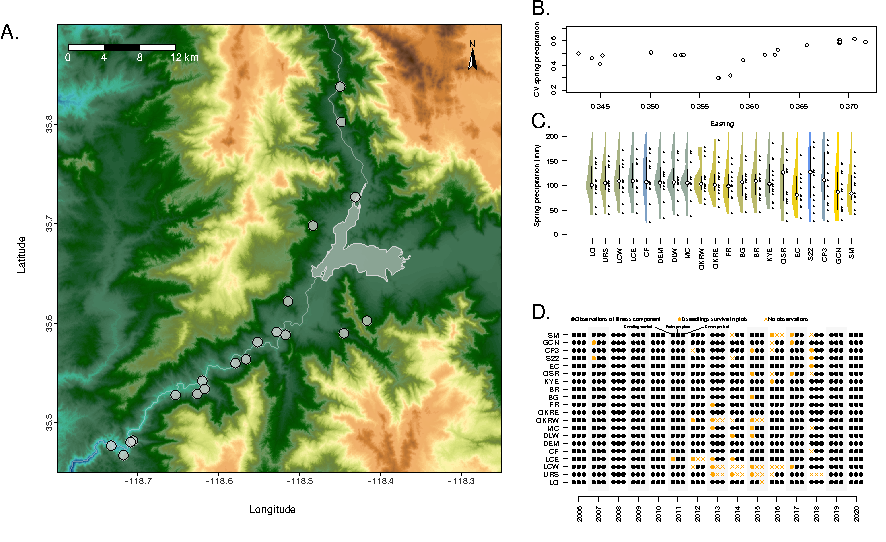
\includegraphics[width=\textwidth]{../manuscript/figures/intro-figure.pdf}  
        \caption{ \footnotesize (A) Elevation map of populations. (B) Coefficient of variation of 15 years of spring (February-June) precipitation plotted against easting. (C) Summary of 15 years of spring precipitation for study populations; study populations are arranged by position on easting. Density plots summarize the distribution of estimates, which are also represented by a point and line showing the median and interquartile range. Fifteen years of estimates are plotted to the left of the summaries. (D) Graphical summary of fifteen years of aboveground observations at study populations. Orange circles indicate that no seedlings survived in permanent plots; orange Xs indicate that no seedlings or plants were observed in surveys. Populations are arrayed from west (bottom) to east (top). }
        \label{fig:intro-figure}
\end{figure}


 \begin{figure}[!h]
\centering
       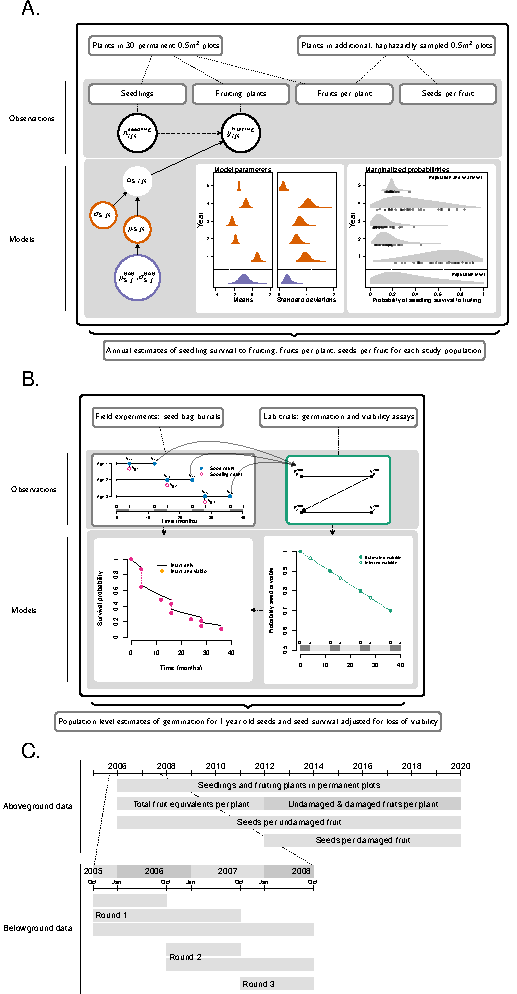
\includegraphics[scale=1]{../manuscript/figures-overview/diagram-figure.pdf}  
 \caption{ Graphical summary of the observations, models, and parameters associated with annual estimates of aboveground components of fitness and population-level estimates of germination and seed survival. (A) A graphical representation of the relationship between the structure of observations and the data. A directed acyclic graph (DAG) for the model of seedling survival to fruiting. Colors of the nodes in the DAG correspond to the distributions in the plots showing the relationship between model parameters, marginalized probabilities, and data. All data in this example are simulated. (B) A graphical representation of the field seed bag experiments and lab viability trials. The experiments are related to estimates of seed survival, germination, and viability. (C) Timeline of the data collected in this study. Aboveground data was collected from 2006-2020; bars are labeled according to when a particular dataset was collected. Belowground experiments were carried out from 2005-2008; bars are labeled according to experimental round. }
   \label{fig:diagram}
 \end{figure}

 \begin{figure}
\centering
\begin{subfigure}[h]{.65\textwidth}
\centering
       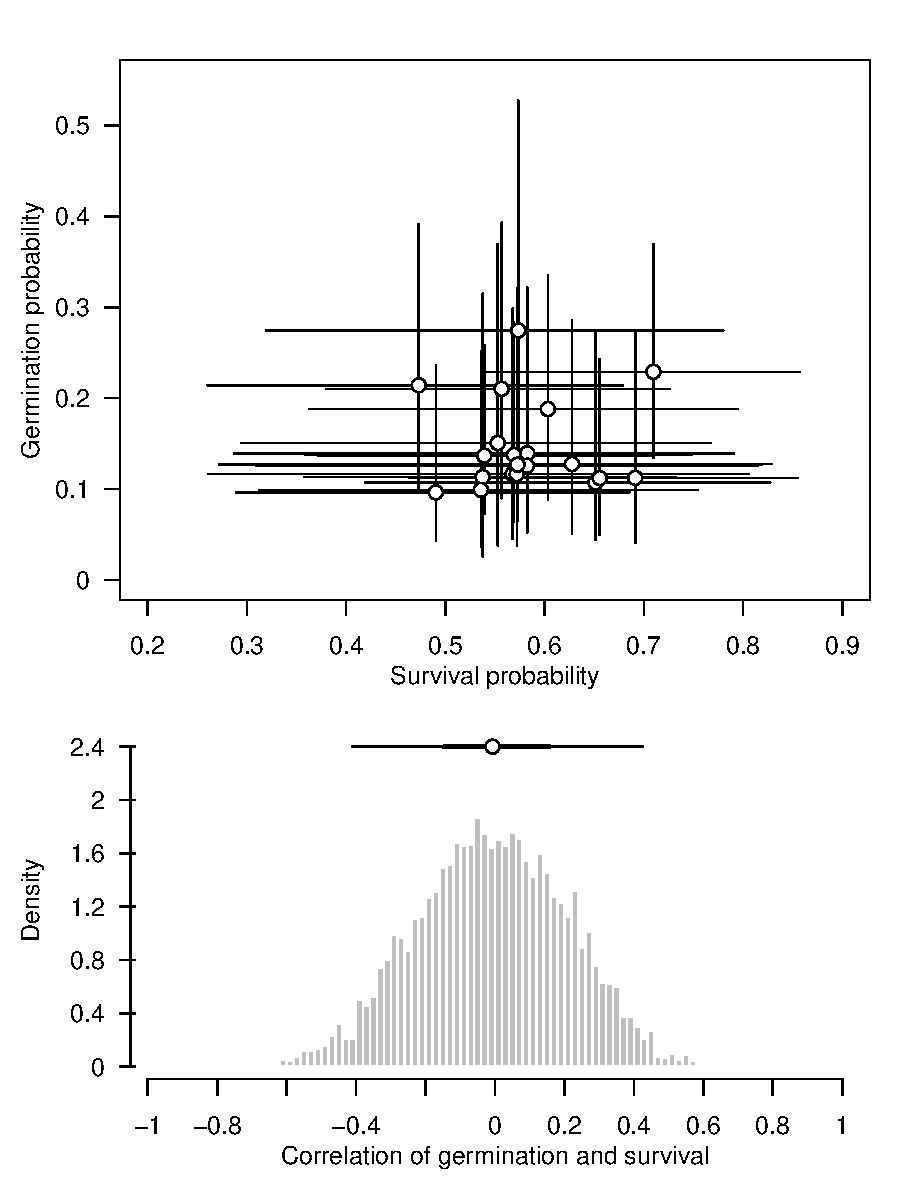
\includegraphics[page=1,width=1\textwidth]{../figures/analysis/correlation-germ-surv.pdf}  
\end{subfigure}
 \caption{ (A) The observed germination probability plotted against probability of seed survival. (B) The posterior distribution of correlation between observed germination probability and the probability of seed survival. }
  \label{fig:correlation-germ-surv}
 \end{figure}
 

 \begin{figure}
\centering
       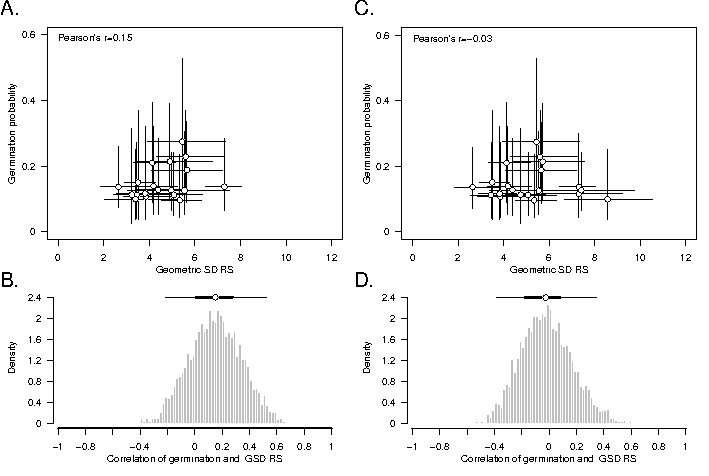
\includegraphics[page=1,width=1\textwidth]{../manuscript/figures/analysis-figure.pdf}  
 \caption{ \textit{Left column}: Correlation between germination and variance in reproductive success when reproductive success is calculated with partial pooling. (A) Observed germination probability plotted against the temporal variation in per capita reproductive success, expressed as geometric standard deviation of per capita reproductive success. (B) The posterior distribution of correlation between observed germination probability and geometric SD of per capita reproductive success. \textit{Right column}: Correlation between germination and variance in reproductive success when reproductive success is calculated with partial pooling, but years without any observed plants are assumed to have reproductive success of zero. Panels (C) and (D) plot the same relationships as in (A) and (B), respectively.}
   \label{fig:obs-pred}
 \end{figure}

 
  \begin{figure}[h]
   \centering
       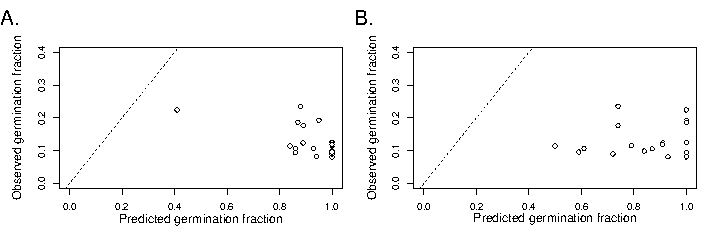
\includegraphics[page=1,width=.9\textwidth]{../manuscript/figures/analysis-figure-2.pdf}  
    \caption{ Comparison of observed and optimal germination probabilities from a density-independent model of bet hedging. (A) Observed vs. predicted probabilities for reproductive success estimated from models with partial pooling. (B) Observed vs. predicted probabilities for reproductive success estimated from models with partial pooling and fitness set to 0 in years without observations. For each population, the observed germination probability is the obtained from the model for seed bank vital rates. Each point is the population-specific median of the posterior of $g_1$ for a model fit to data from seed bag experiments from 2006--2009. Data was pooled across years. The dotted line indicates a 1:1 relationship between observations and predictions. Values below the line indicate that the model predicts higher germination probabilities than observed; values above the line would indicate that the model predicts lower germination probabilities than observed. }
 \label{fig:obs-pred-lowFitness}
\end{figure}

\begin{figure}[!h]
       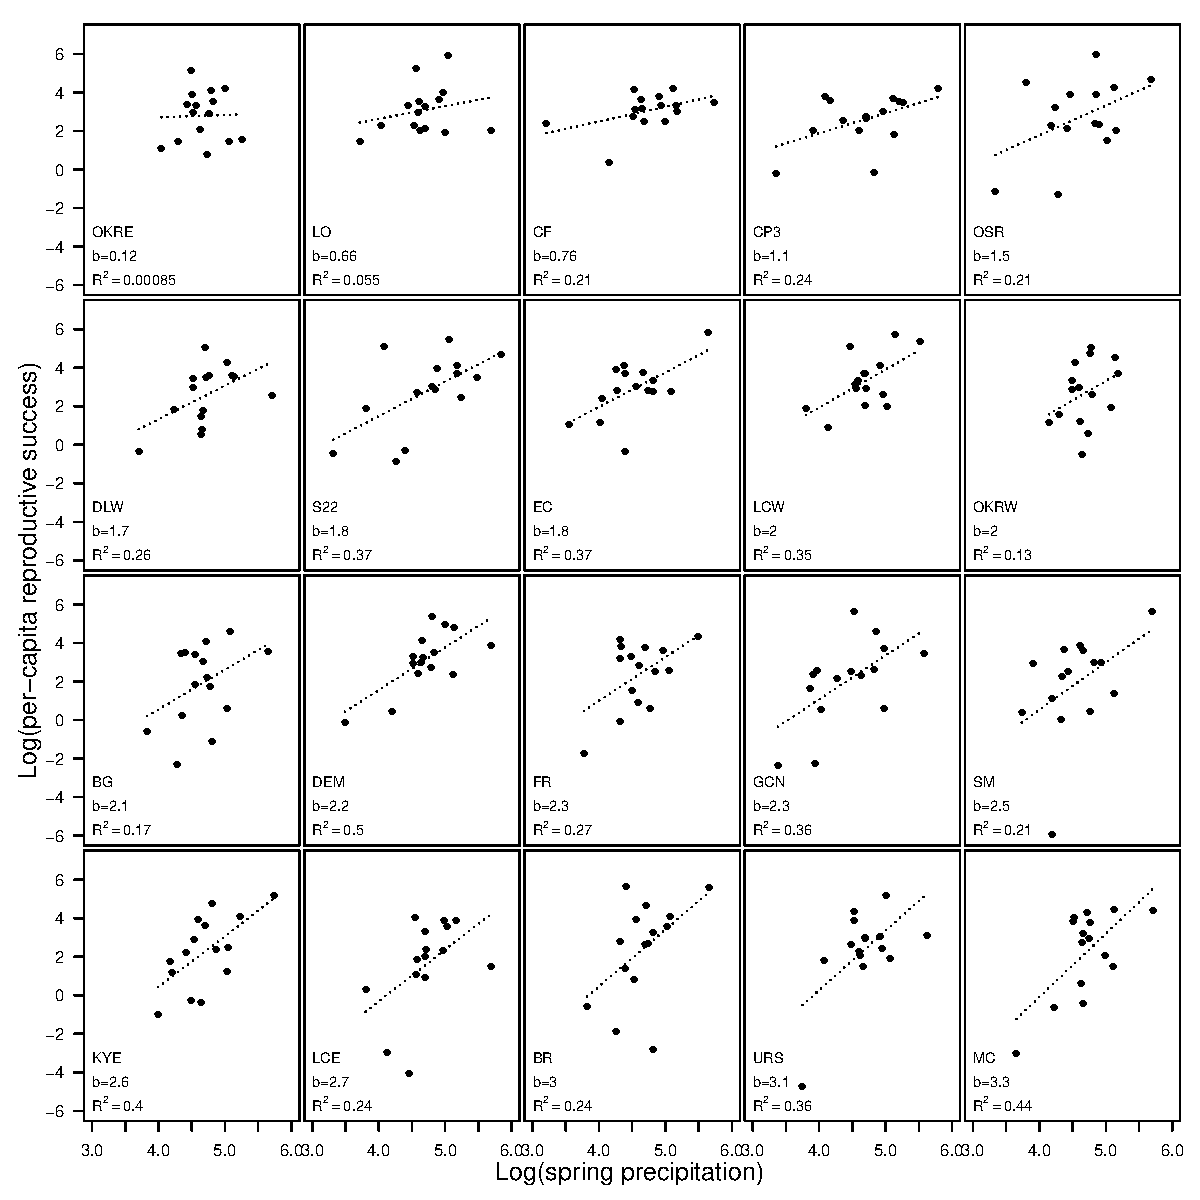
\includegraphics[width=\textwidth]{../figures/analysis/rs-climate-sensitivity.pdf}  
    \caption{ Log of per-capita reproductive success plotted against log of cumulative growing season (spring) precipitation. Plots are arrayed by easting from west to east, with the most western populations at the top left and the most eastern populations at the bottom right. }
       \label{fig:climate-sensitivity}
\end{figure}

\begin{figure}[!h]
       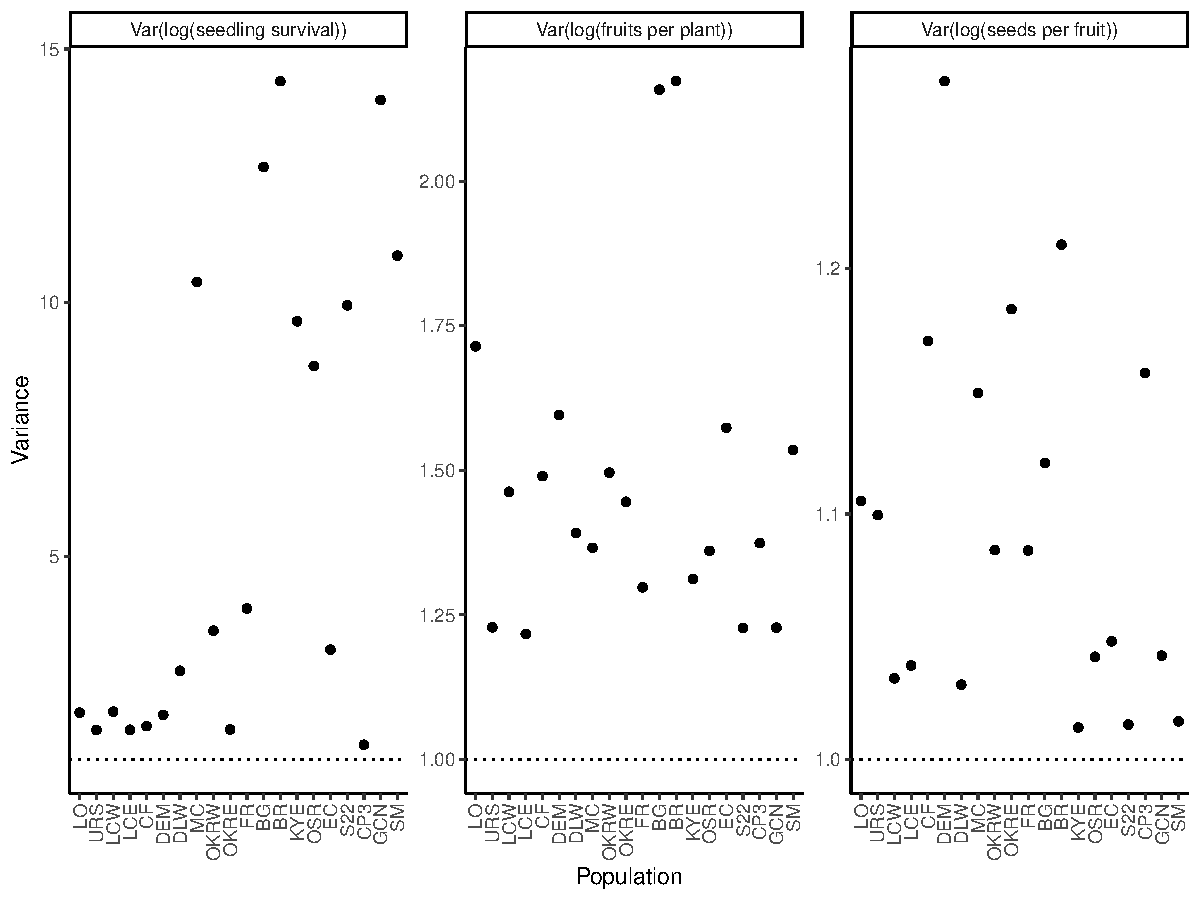
\includegraphics[width=\textwidth]{../figures/analysis/variance-decomp.pdf}  
    \caption{ Variance of the log of fitness components. Per-capita reproductive success and its components (seedling survivorship, fruits per plant, seeds per fruit) were summarized by their medians, and decomposed to assess the relative contribution of variance in each component to total geometric variance. The dotted line corresponds to $\exp(0)=1$, the level at which the component makes no contribution to total geometric variance. Plots are arrayed by easting from west to east. The y-axis in each panel differs. }
       \label{fig:variance-decomposition}
\end{figure}

\clearpage
%%%%%%%%%%%%%%%%%%%%%%%%%%%%%%%%%%%%%%%%%%%%%%%%%%%%
% BIBLIOGRAPHY
%%%%%%%%%%%%%%%%%%%%%%%%%%%%%%%%%%%%%%%%%%%%%%%%%%%%
\bibliographystyle{/Users/gregor/Dropbox/bibliography/styleFiles/ecology} 
\bibliography{/Users/gregor/Dropbox/bibliography/chapter-1}

\clearpage
%%%%%%%%%%%%%%%%%%%%%%%%%%%%%%%%%%%%%%%%%%%%%%%%%%%%
% SUPPLEMENTARY MATERIAL
%%%%%%%%%%%%%%%%%%%%%%%%%%%%%%%%%%%%%%%%%%%%%%%%%%%%
\section*{Supplementary material}

%\subsection*{Theoretical background for hypotheses.} Explanation of key papers that develop theoretical results about seed banks. The document describes results from these papers that are relevant to understanding and interpreting the data in this manuscript. Link to document: \url{https://github.com/gregor-fausto/clarkiaSeedBanks/blob/master/products/appendices/appendix-cohen-results/appendix-x-cohen-results.pdf}

\subsection*{Data summary.} Summary tables for all datasets used in the manuscript. The document summarizes the types of data collected. The document provides a table summarizing each dataset (e.g. sample size per each site and year). Link to document: \url{https://github.com/gregor-fausto/clarkiaSeedBanks/blob/master/products/tables/data-summary.pdf}

\subsection*{Parameter estimation.} Description of all models used to estimate demographic parameters. Link to document: \url{https://github.com/gregor-fausto/clarkiaSeedBanks/blob/master/products/tables/data-summary.pdf}

\subsection*{Joint posterior.} Expression for the posterior proportional to the joint distribution, and corresponding directed acyclic graphs. Link to document: \url{https://github.com/gregor-fausto/clarkiaSeedBanks/blob/master/products/appendices/appendix-joint-posteriors/appendix-joint-posteriors.pdf}

\subsection*{Priors.} Explanation of priors. Link to document: \url{https://github.com/gregor-fausto/clarkiaSeedBanks/blob/master/products/appendices/appendix-priors/appendix-priors.pdf}

\subsection*{Model checks.} Model checks, including visual posterior predictive checks and assessments with Bayesian $p$-values for test statistics. Link to document: \url{https://github.com/gregor-fausto/clarkiaSeedBanks/blob/master/products/appendices/appendix-model-checks/appendix-x-model-checks.pdf}

\end{document}